\documentclass[a4paper,12pt]{report}

\usepackage{alltt, fancyvrb, url}
\usepackage{graphicx}
\usepackage[utf8]{inputenc}
\usepackage{float}
\usepackage{hyperref}
\usepackage[italian]{babel}
\usepackage{appendix}
\usepackage[italian]{cleveref}
\usepackage{xcolor}
\usepackage{microtype}
\usepackage{array}
\usepackage{adjustbox}
\usepackage{tabularx}
\usepackage{colortbl}
\usepackage{pdfpages}
\usepackage{listings}
\usepackage{booktabs}
\usepackage{longtable}
\usepackage{xltabular}
\usepackage{ulem}

\lstdefinestyle{codeStyle}{
    basicstyle=\small\ttfamily,
    keywordstyle=\color{blue},
    commentstyle=\color{green},
    stringstyle=\color{red},
    numbers=left,
    numberstyle=\tiny\color{gray},
    frame=single,
    breaklines=true,
    tabsize=4
}
\lstset{}
\newcolumntype{C}{>{\centering\arraybackslash}X}
\newcolumntype{D}{>{\center\arraybackslash}X}

\newcommand{\speciallabel}[2]{
	% \speciallabel{<stuff>}{<label>}
  \edef\@currentlabel{#1}\label{#2}%
}

\newcommand{\tableheader}{% % il comando prende quattro argomenti
\hline % disegna una linea orizzontale
\rowcolor{red} % colora la riga di rosso
\multicolumn{1}{|C|}{\textcolor{white}{\uppercase{concetto}}} & % centra e mette in grassetto il primo argomento
\multicolumn{1}{C|}{\textcolor{white}{\uppercase{costrutto}}} & % centra e mette in grassetto il secondo argomento
\multicolumn{1}{C|}{\textcolor{white}{\uppercase{accessi}}} & % centra e mette in grassetto il terzo argomento
\multicolumn{1}{C|}{\textcolor{white}{\uppercase{tipo}}} \\ % centra e mette in grassetto il quarto argomento
\hline % disegna una linea orizzontale
}

% A new counter for the rows
\newcounter{rowcntr}[table]
\renewcommand{\therowcntr}{\table\number\numexpr\value{rowcntr}\relax}


% A new columntype to apply automatic stepping
\newcolumntype{N}{>{\refstepcounter{rowcntr}\therowcntr}l}

% Reset the rowcntr counter at each new tabular
\AtBeginEnvironment{tabular}{\setcounter{rowcntr}{0}}


\graphicspath{{../resources/img}}
\title{Elaborato Basi di Dati}
\author{Desiderio Edoardo}
\begin{document}
\maketitle
\titlepage
\tableofcontents
\newpage

\chapter{Analisi dei requisiti}
Lo scopo è realizzare un portale che permetta alla società richiedente di gestire in maniera informatizzata le prenotazini e l'organizzazione
delle visite guidate che vuole organizzare con i siti di maggior interesse.
\section{Intervista}
Una	 società	 operante	 nel	 settore	 del	 turismo	 offre	 tra
i	 suoi	 servizi	 l’organizzazione	 di	 	 visite guidate	a	siti
d' interesse	storico-culturale. Ogni	visita,	opportunamente	descritta,	ha
un	 titolo	 (diverse	visite	hanno	un	 titolo	 ricorrente,	es. “Musei
Vaticani	e	Cappella	Sistina”,	“Sito	archeologico	di	Pompei”,
“Galleria	degli	uffizi”,	ecc.),	la sua	durata	media		e	il
luogo		in	cui	essa	si	svolge.	Ogni	visita	può	avere	luogo	più
volte	nel	tempo secondo	specifici	eventi	programmati. Le escursioni,	di
cui	viene	indicato	il	prezzo,	vengono	prenotati	da	gruppi	di	persone
condotti	da	una guida	che	illustra	il	percorso	in	una	determinata
lingua;	per	ogni	gruppo	viene	fissata	l’ora	d' inizio della	visita	e un
numero	minimo	e	massimo	di	partecipanti. Il prezzo degli eventi varia in
base all'età:
\begin{itemize}
	\item 0-12 il prezzo è gratuito
	\item 12-14 il prezzo è scontato del 20\%
	\item gli over 50 godono di uno sconto pari al 10\%
\end{itemize}
La	società	si	avvale	di	diverse	guide	ognuna	delle	quali	ha
competenze	in	una	o	più	lingue	ad uno specifico	 livello	 di
conoscenza	 ("B2","C1","C2"). Di ogni capo gruppo	 si	 vuole conoscere
alcuni	 dati	 tra	 i	 quali	 nome,	 sesso,	 data	 di	 nascita,
titolo	 di	 studio	 e	 relativo	 anno	 di conseguimento. \\
I	clienti,	di	cui	si	vuole	conoscere	almeno	nome,	nazionalità,
lingua	base,	e-mail	e	un	 recapito telefonico,	 possono	 aggregarsi
a	 uno	 o	 più	 gruppi,	 secondo	 le	 loro	 esigenze.	 Uno
stesso visitatore,	 nel	 tempo,	 può	 partecipare	 a	 gruppi	 diversi
usando	 ogni	 volta	 una	 certa	 forma	 di pagamento	(non
necessariamente	sempre	la	stessa	es.	Carta	di	credito,	paypal,	bonifico
bancario) della	quale	si	deve	prevedere	la	memorizzazione:	tipologia,
descrizione	e	data	del	pagamento. Il	 sito	 web	 della	 società
consente	 la	 visione	 pubblica	 delle	 visite	 organizzate	 e,
solo	 agli	 utenti preventivamente	registrati,	la	prenotazione	di	una
specifica	visita. In fine l'applicativo deve permettere una visione protetta
dei dati, quindi non tutti gli utenti ad esempio possono visionare i gruppi a
cui sono affidate le guide

\section{Rilevamento delle ambiguità e correzioni proposte}
Il testo dell'intervista presenta molte ambiguità. Le principali sono
\begin{itemize}
	\item utilizzo di sinonimi
	\item Elenchi di attributi incompleti
	\item Cartdinalità non specificate
\end{itemize}

Gli attributi parziali e le cardinalità verranno risolti mediante l'uso della logica in fase di creazione dello schema concettuale.
Invece per quanto concerne i sinonimi, è necessario costruire un glossario dei termini


\begin{table}[H]
	\begin{center}
		\begin{tabularx}{\textwidth}{|C|C|C|C|}
			\hline
			\rowcolor{red} \textcolor{white}{termine} & \textcolor{white}{descrizione}                                             & \textcolor{white}{sinonimi} & \textcolor{white}{collegamenti} \\
			\hline
			utente                                    & entità che interagisce con il database lato consumatore                    & cliente, visitatore         & gruppi, pagamenti, sconti       \\
			\hline
			guida                                     & figura qualificata in lingue e storia che illustra il percorso passo passo & capo gruppo, dipendente     & competenze linguistiche, gruppi \\
			\hline
			sconto                                    & rappresenta la percentuale da decurtare al prezzo finale in base all'età   & -                           & pagamento, cliente              \\
			\hline
			gruppo                                    & insieme di persone in questo caso                                          & -                           & cliente, guida, evento          \\
			\hline
			evento                                    & situazione specifica dato un luogo e orario                                & visita-guidata, escursioni  & visita, gruppi                  \\
			\hline
			visite                                    & logo d'interesse con cui ha accordi la società di turismo                  & sito culturale              & eventi                          \\
			\hline
		\end{tabularx}
		\caption{\label{glossario:termini}} termini rappresentativi dell' intervista
	\end{center}
\end{table}


\subsection*{Ipotesi aggiuntive}
dall'intervista fatta si concretizza che:
\begin{itemize}
	\item il dato relativo alla durata media di una visita venga espresso in
	      minuti
	\item  per	uno	specifico	evento	di	visita	guidata	possano	essere
	      formati	anche	più	gruppi		ognuno col	proprio	orario,
	      accompagnatore	e	lingua;
	\item i	 vari	 visitatori	 per	 potersi	 iscriversi	 ad	 uno	 o
	      più	 eventi	 debbono	 registrarsi	 sul	 sito	 della
	      società	 fornendo	 e-mail	 e	 password.	 La	 banca	 dati	 non
	      prevede	 alcuna	 gestione relativamente	 agli	 utenti	 anonimi:
	      essi	 possono	 operare	 solo	 per	 funzionalità
	      limitate	 d' interrogazione	per	vedere	i	dati	degli	eventi
	      programmati;
	\item per	potersi	iscrivere	ad	un	gruppo	di	visita	relativamente
	      ad	uno	specifico	evento,	nei	limiti della	 disponibilità	 di
	      posti,	 ogni	 visitatore	 registrato	 effettui	 il	 pagamento
	      tramite	 carta	 di credito	 (con	 codice	 della	 medesima),	 via
	      PayPal	 (l’utente	 deve	 essere	 registrato	 a	 tale servizio),
	      o	 tramite	 bonifico	 bancario	 di	 cui	 deve	 fornire
	      gli	 estremi	 utilizzando	 il	 campo relativo	alla
	      descrizione	del	pagamento;
	\item il	prezzo	di	una	visita	sia	comunque	individuale	e	venga
	      espresso	a	livello	di	evento	in	quanto suscettibile	di
	      variazioni	nel	tempo
	\item per definire `gratuito' il prezzo di un biglietto si imposterà una
	      percentuale di sconto pari al 100\%
\end{itemize}


\newpage
\section{Definizione delle specifiche in linguaggio naturale ed estrazione dei concetti principali}
Di seguito si riporta un testo riassuntivo in cui sono evidenziati i concetti
chiave dell’ intervista filtrati dalle ambiguità possibili, in modo da avere un’
idea più chiara di quelle che saranno le entità presenti nello schema
concettuale.\\\\
La società commissionatrice vuole creare la gestione informatizzata dei suoi
servizi.\\
Ogni \textbf{\underline{visita}}, intesa come il sito culturale è opportunamente
descritta definendo il titolo, luogo, identificativo, descrizione, durata media
espressa in minuti.\\
Per ogni visita la società organizza degli eventi. Ogni
\textbf{\underline{evento}} può ripetersi più volte rispetto ad una determinata
visita e ne viene definito il prezzo indicato che può variare nel tempo; si
vuole memorizzare anche la data dell'evento.\\\\
I \textbf{\underline{clienti}}, di cui si salvano lingua preferenza e dati
principali una password e mail per accedere a funzionalità più avanzate per la
prenotazione di biglietti ecc, vengono assegnati a gruppi differenti in base
alle loro preferenze proposte  al momento dell'acquisto dei \textbf{biglietti}.
Per gestire i pagamenti il cliente potrà aggiungere al carrello i biglietti che
intende acquistare per poi procedere al pagamento utilizzando quello che più
preferisce (paypall, bonifico, carta di credito) \\\\
Dei \textbf{\underline{Gruppi}} si vuole indicare l'orario d' inizio della
visita si vuole specificare il minimo numero di persone da cui deve essere
composto un gruppo e il massimo, bisogna valutare se è conveniente salvare anche
il numero d' iscritti correnti o lasciare il dato deducibile.\\\\
I \textbf{\underline{biglietti}} devono essere acquistati dall'utente, siccome
ogni utente può acquistare biglietti anche per altre persone ogni biglietto deve
specificare il nome e il cognome e l'età della persona per cui viene acquistato
il biglietto siccome sono previste fasce di \textbf{\underline{sconto}} in base
all'età. Rispettivamente \(eta \le 12 \rightarrow\)  100\%, \(12 < eta \le 14
\rightarrow\)  20\%, \(eta >50 \rightarrow\)  10\%. Per ogni nuovo evento
vengono emessi biglietti pari al numero minimo di partecipanti di un gruppo\\\\
IL \textbf{\underline{carrello}} deve raccogliere le registrazioni per biglietti
a persona per poi calcolare il totale dell'ordine. A livello applicativo sarà
gestito da una vista che assocerà gli ordini fatti dal cliente \\\\
Delle \textbf{\underline{guide}} turistiche oltre ai dati comuni con il cliente
si vuole memorizzare anche il titolo di studio e il suo anno di conseguimento.
La società intende registrare i dati relativi alle
\textbf{\underline{competenze}}. Ogni competenza deve essere riferita ad una
guida e alle lingue che essa conosce, il livello di conoscenza deve essere
espresso in (B2,C1,C2).

\section*{Individuazione operazioni principali}\label{sec:operazioni}
\begin{enumerate}
	\item Aggiunta di visite
	\item Aggiunta di eventi
	\item inserimento di un nuovo cliente
	\item inserimento di una nuova guida
	\item supponendo che le guide si specializzino in altre lingue aggiunta di una nuova competenza di una guida
	\item gestione e riepilogo ordini
	\item Aggiunta di un nuovo gruppo
	\item creazione di biglietti fino al numero minimo di partecipanti ad un gruppo
	\item vendita di biglietti per un determinato cliente
	\item applicazione sconto in base al destinatario del biglietto acquistato
	\item storico degli acquisti
	\item controllo del riempimento dei gruppi
	\item assegnazione di una determinata guida ad un gruppo in base alle sue conoscenze
	\item indicazione dei posti rimanenti per le iscrizioni ad un gruppo
	\item aggiunta di una nuova lingua
	\item inserimento di un nuovo metodo di pagamento
	\item modifica valori Biglietto
	\item creazione vista dello storico ordini per ogni cliente
	\item Ricerca filtrata di annunci di visite da
	      acquistare in base a diversi parametri scelti
	\item ricerca delle visite disponibili in base ad una data
\end{enumerate}
vedi stima frequenza piú avanti\ref{sec:frequenza}
\newpage
\chapter{Progettazione concettuale}
Per maggiore chiarezza, di seguito riportiamo i primi esempi di schemi concettuali
divisi per ambiti. Partirò da parti di schema concettuale più semplici fino ad arrivare a parti più complesse
\subsection*{Visita-Evento-Gruppo}
\begin{figure}[H]
	\centering
	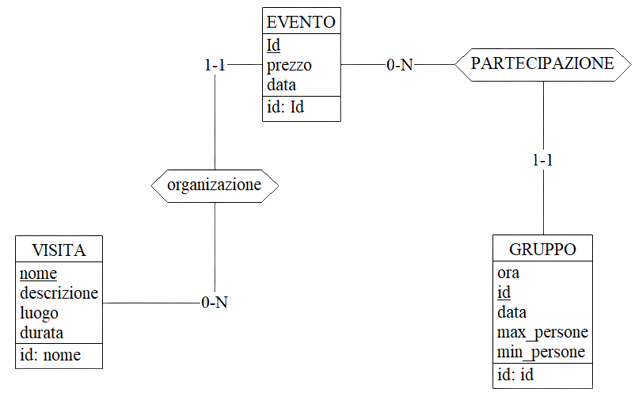
\includegraphics[width=0.99\textwidth]{evento-visita-gruppo.png}
	\caption[]{caratterizzazione della gestione fra le visite, i vari eventi che può ospitare e i gruppi che vi partecipano}
\end{figure}
Lo schema è piuttosto auto esplicativo, sono stati mantenuti i vincoli imposti
dall'intervista come permettere l'Associazione di più eventi data una visita e
la partecipazione di più gruppi al determinato evento si noti come da un gruppo
si possa risalire ad un determinato evento e ad una determinata visita.
\subsection*{Gerarchia persone, relazione fra gruppi guide e competenze}
\begin{figure}[H]
	\centering
	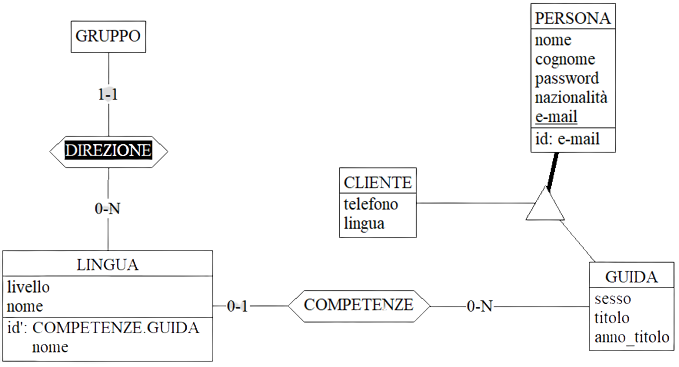
\includegraphics[width=0.99\textwidth]{gruppo-guide.png}
	\caption[]{l'entità gruppo è descritta nella figura sopra}
\end{figure}

Per gestire le entità CLIENTE, GUIDA poiché ave\-vano campi
simili ho optato per una gerar\-chia di tipo totale ed Esclusiva
( DB\_MAIN non mostrava la scritta t, e)\-.
Il resto dello schema E-R portato esplicita la modellazione di associare
più tipi di lingue ad una determinata guida. Lingua quindi è un'entità debole
che necessita della chiave di GUIDA per essere completa. Adottando questo metodo
per ogni gurppo posso risalire alla guida e con che lingua e a che livello sarà
diretto.

\subsection*{Biglietto-Ordine-Cliente}

\begin{figure}[H]
	\centering
	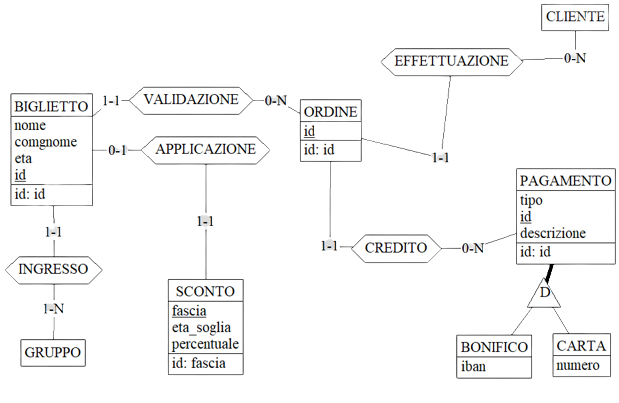
\includegraphics[width=0.99\textwidth]{BIGLIETTO-ORDINE.png}
	\caption{i biglietti rappresentano il punto di collegamento relazionale fra i gruppi e i clienti}
\end{figure}

Per ogni gruppo è previsto che verranno pubblicati N biglietti in base al numero
minimo di posti destinabili ad un gruppo. Viste le richieste del testo ho deciso
di rendere personale il biglietto e dividere l'acquirente dal proprietario. Lo
sconto va verificato per ogni biglietto e il suo acquirente, le fasce di prezzo
sono predefinite. Un ordine può riferirsi a più biglietti, in questo modo il
cliente potrà acquistare più biglietti. Per il pagamento è stata generata una
gerarchia parziale ed esclusiva poiché il pagamento con paypall sarebbe un link
al sito e si potrebbe benissimo gestire direttamente lato software.

\section{Schema scheletro}
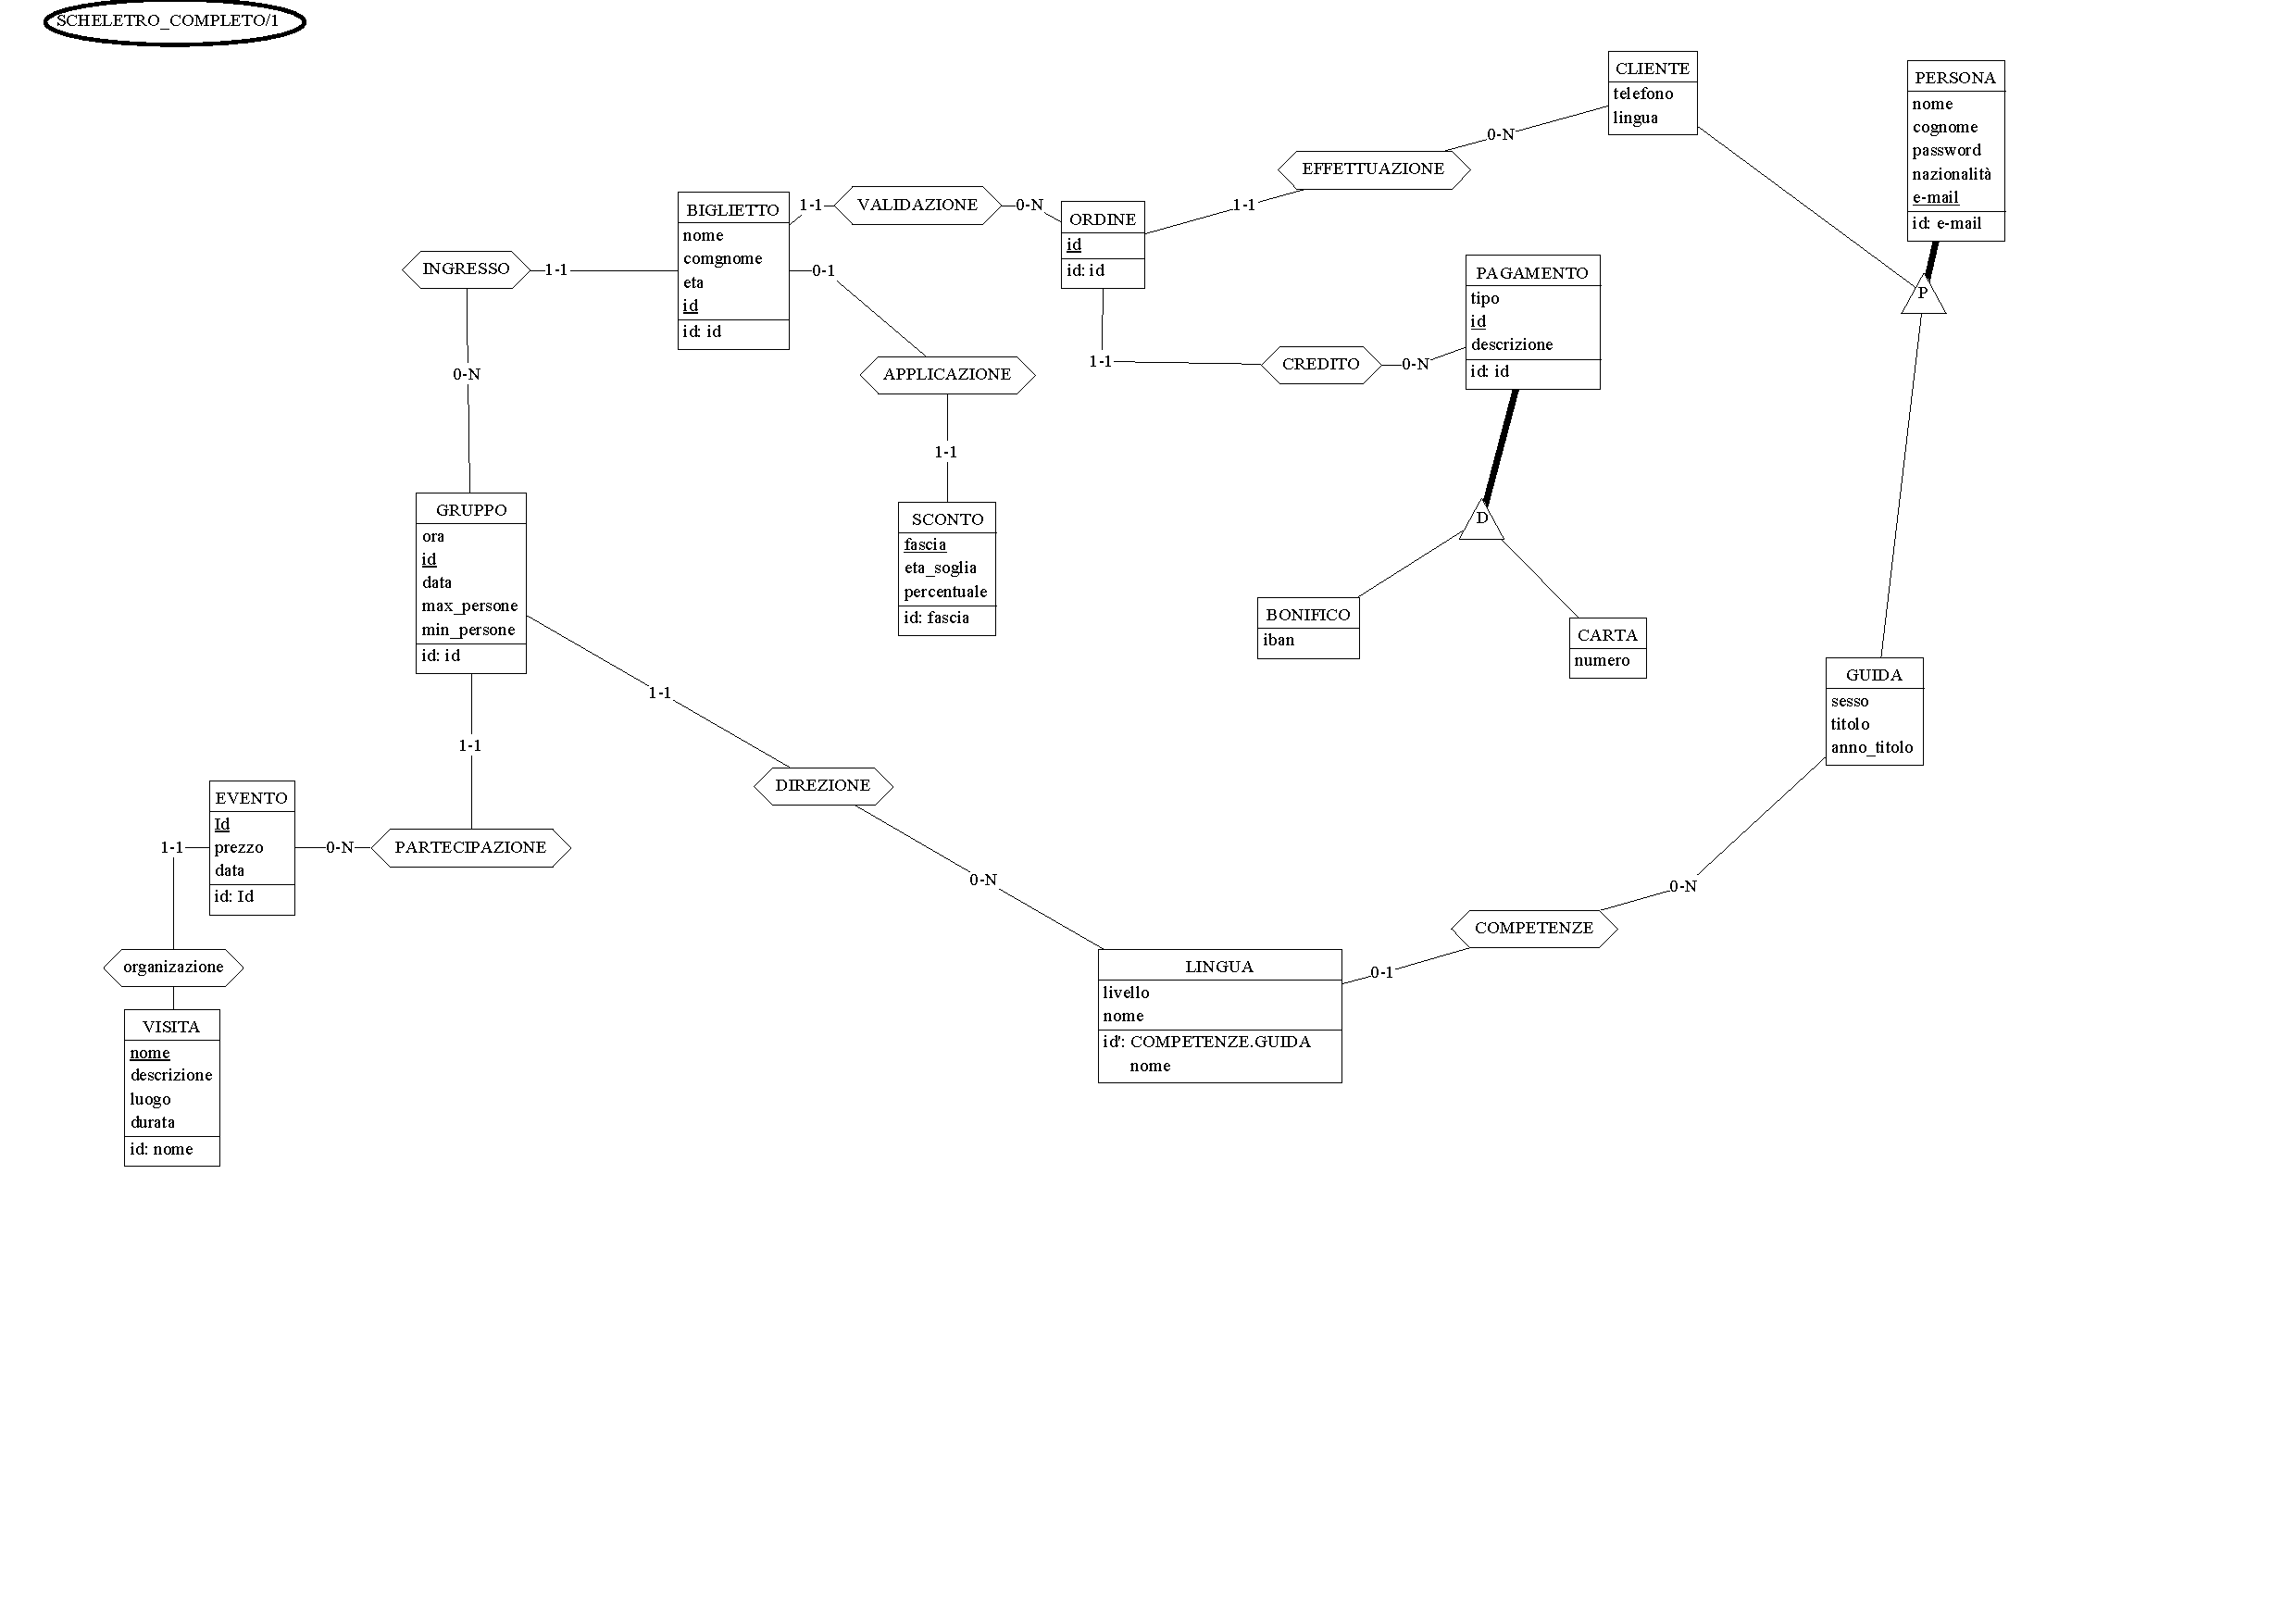
\includepdf[angle=90]{../resources/pdf/SCHELETRO2.pdf}

\section{Raffinamenti proposti}
Come si nota dagli schemi riportati, esistono attributi di qualche tabella che
sarebbe meglio modellare come entità indipendenti. In Particolare:
\begin{itemize}
	\item L'attributo `lingua' dell'entità cliente verrà modellato come entità
	      nuova nello schema contenente tutte le lingue che il dominio del problema
	      dovrà trattare
	\item l'entità lingua diventerà `COMPETENZA', sarà un'entità debole poiché
	      avrà come super-chiave il riferimento esterno alla lingua e alla guida.
	\item l'attributo `tipo' presente nell' entità  `PAGAMENTO' sarà gestito a
	      parte in modo da definirne i metodi di pagamento supportati. l'entità si
	      chiamerà `METODO' così facendo posso eliminare la gerarchia nata da pagamento
	\item la relazione `CREDITO' ora conterrà un attributo prezzo
	\item corretta la cardinalità fra sconto e biglietto (0-N) considerando che un tipo di sconto
	      potrebbe essere legato a più biglietti
\end{itemize}
La trasformazione di questi attributi in entità comporta numerosi vantaggi:
diminuisce gli errori in fase d'inserimento e limita il dominio possibile di
questi attributi alle sole istanze presenti nelle relative entità.



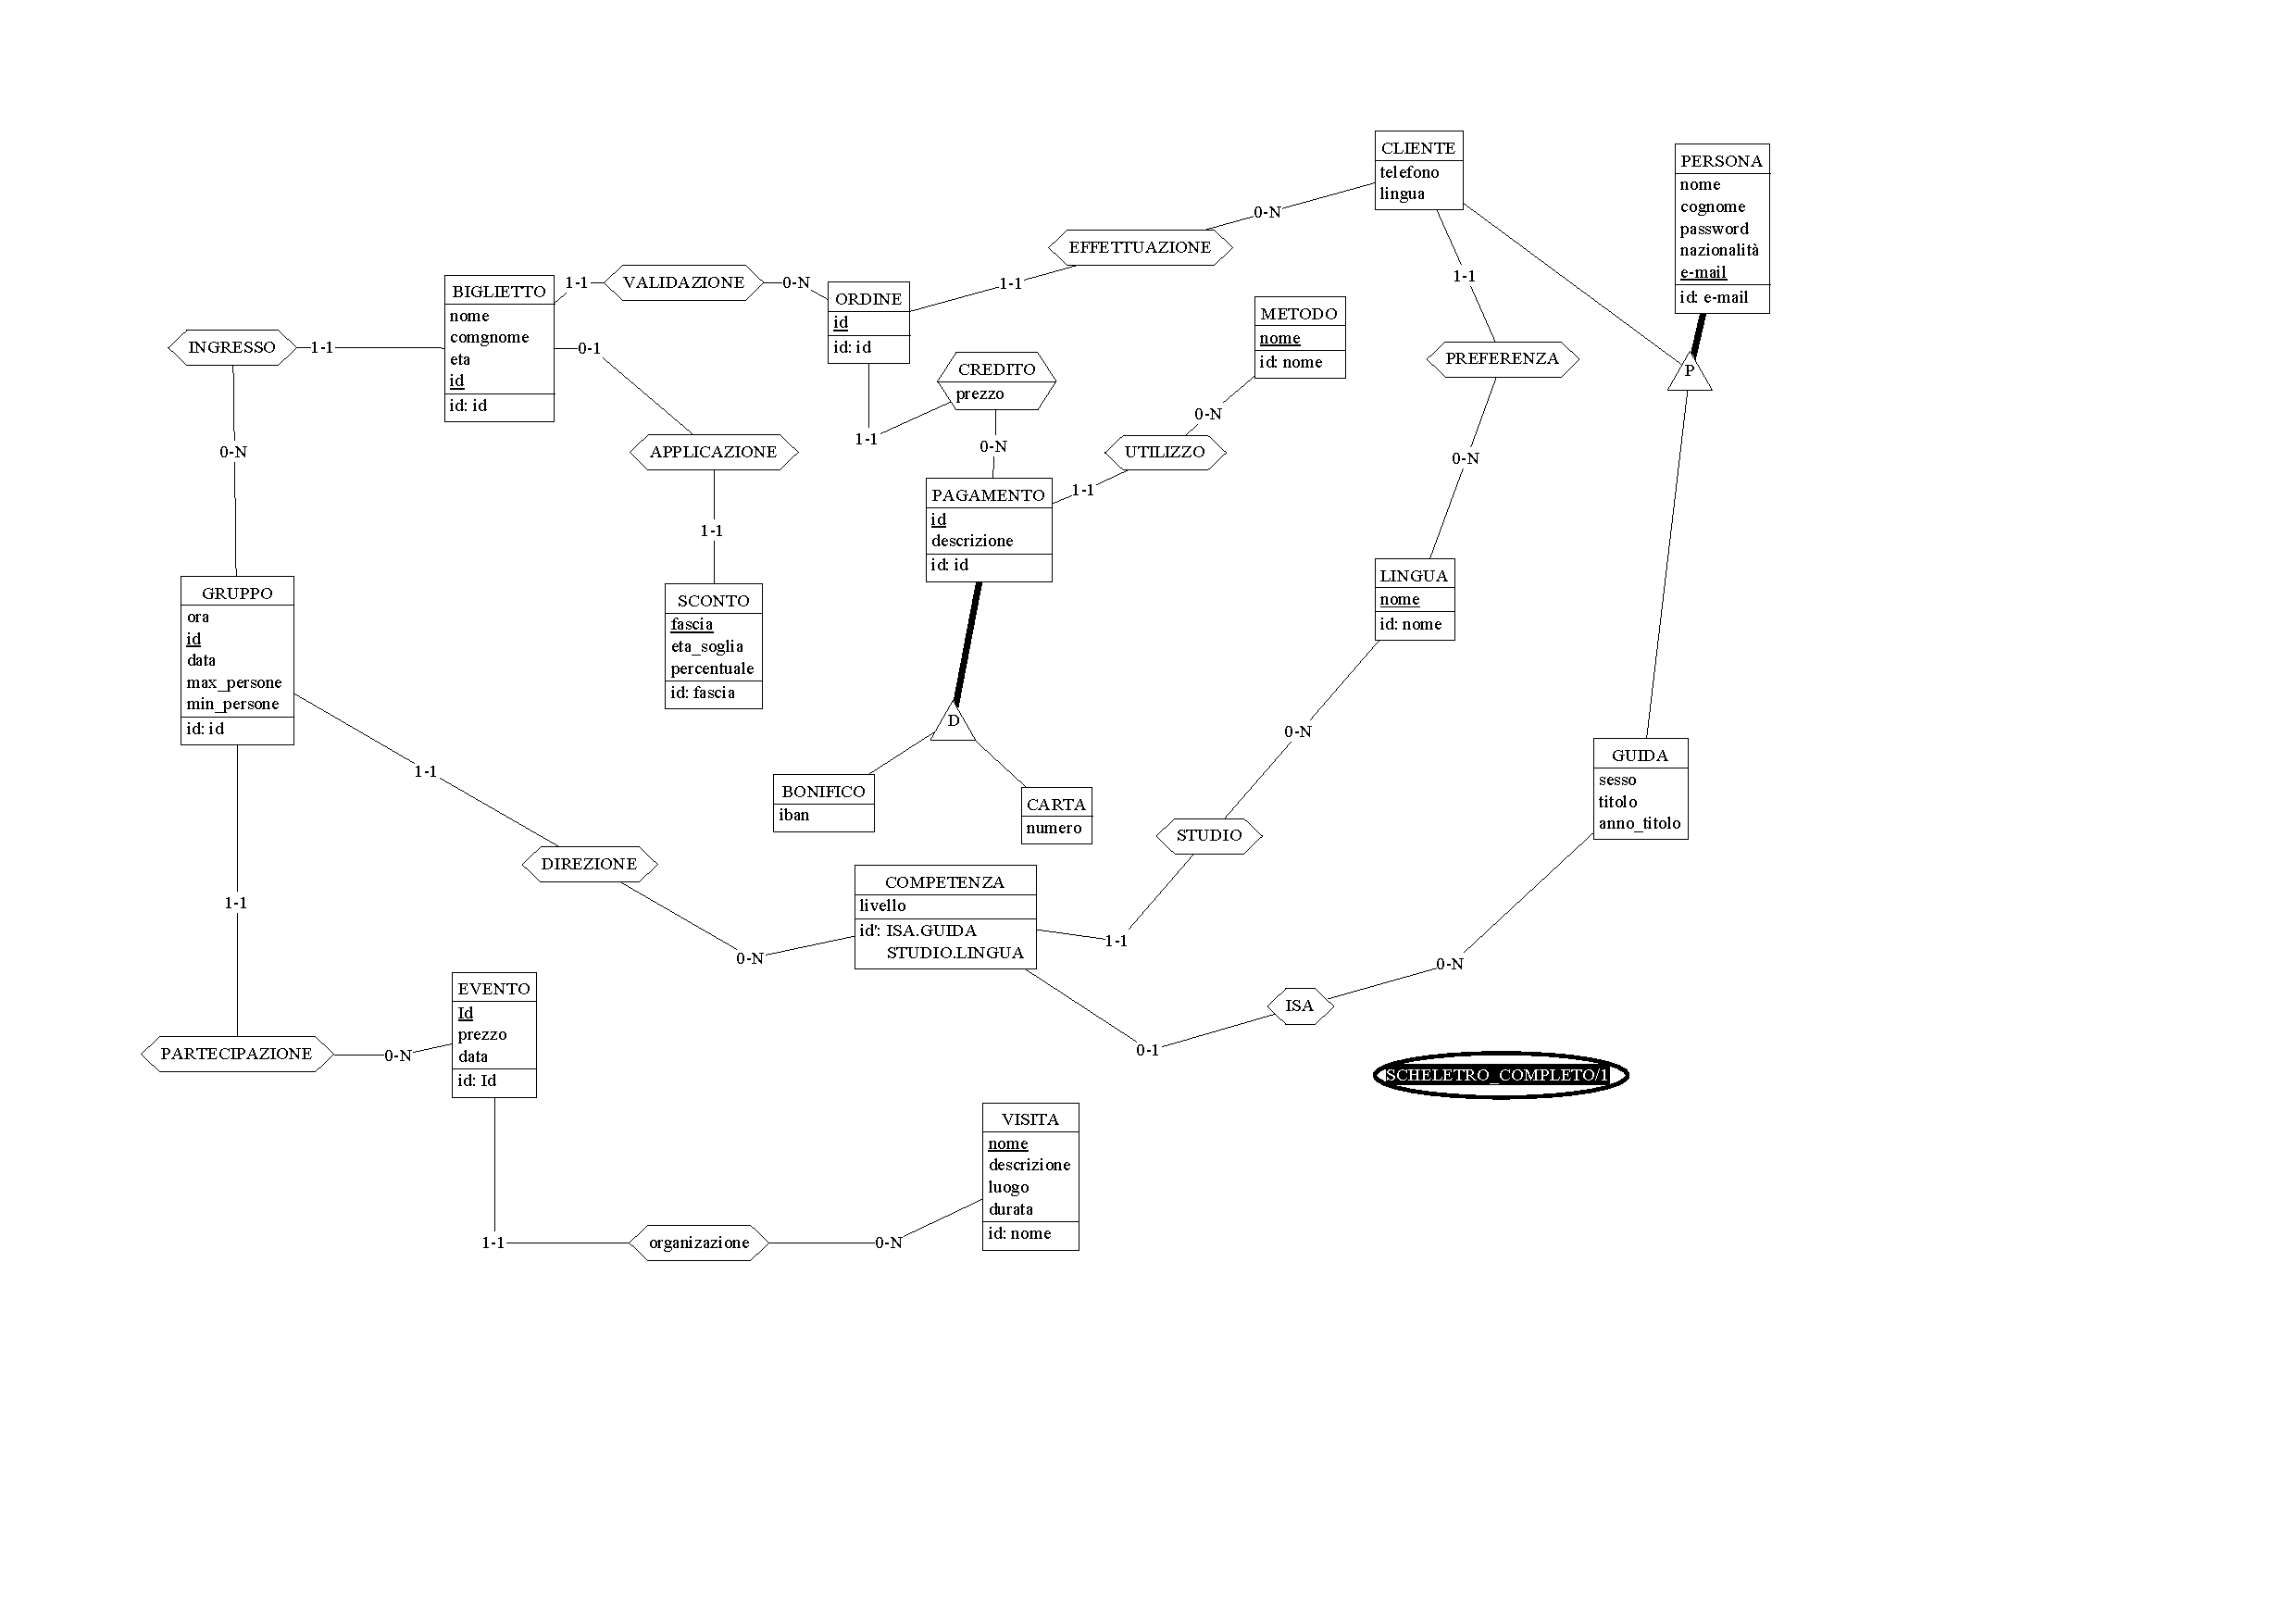
\includepdf[angle=90,pagecommand=\section{Schema concettuale finale}\thispagestyle{empty}]{../resources/pdf/raffinamento2.pdf}
\newpage
\chapter{Progettazione logica}
\section{Stima del volume dei dati}
Nella tabella di seguito è riportato il volume atteso per ciascun costrutto
presente nello schema concettuale. Per maggiore chiarezza, rispetto alla
classica tabella che si usa per la stima dei volumi è stata aggiunta una colonna
per descrivere brevemente alcuni costrutti dal nome ambiguo (specialmente
associazioni), in modo da avere immediatamente idea dell’oggetto di cui si sta
parlando senza dover trovare il riferimento nello schema concettuale. Inoltre,
per garantire maggiore compattezza sono state omesse le stime dei volumi delle
associazioni 1-N, in quanto equivalenti ai volumi delle entità che partecipano
alle associazioni stesse con cardinalità 1.


\begin{xltabular}{\textwidth}{|D|D|D|D|}
	\caption{Volume dei dati} \label{tab:volumeDati}\\
	\hline
	\rowcolor{red} \textcolor{white}{\uppercase{concetto}} & \textcolor{white}{\uppercase{costrutto}} & \textcolor{white}{\uppercase{volume}} & \textcolor{white}{\uppercase{descrizione}} \\
	\hline
	\endhead
	\uppercase{cliente}                 & \uppercase{e}         & 100000             & registrazioni di utenti curiosi                                                       \\
	\hline
	\uppercase{biglietto}               & \uppercase{e}         & 80000              & i biglietti sono 80\% degli utenti iscritti                                           \\
	\hline
	\uppercase{ordine}                  & \uppercase{e}         & 26000              & in media un ordine acquista 3 biglietti quindi \(\frac{80000}{3}\)                                  \\
	\hline
	\uppercase{gruppo}                  & \uppercase{e}         & 16000              & considero una media di 5 persone a gruppo                                             \\
	\hline
	\uppercase{evento}                  & \uppercase{e}         & 3200               & ad ogni evento partecipano 5 gruppi                                                   \\
	\hline
	\uppercase{sconto}                  & \uppercase{e}         & 13334              & la frequenza degli sconti sono pari ad \(\frac16\)                                    \\
	\hline
	\uppercase{visite}                  & \uppercase{e}         & 640                & per ogni visita ci sono 5 eventi                                                      \\
	\hline
	\uppercase{pagamento}               & \uppercase{e}         & 13000              & ogni 2 ordini viene usato lo stesso metodo                                            \\
	\hline
	\uppercase{metodo}                  & \uppercase{e}         & 10                 & ad esagerare prevedo 10 metodi diversi per il pagamento                               \\
	\hline
	\uppercase{lingua}                  & \uppercase{e}         & 25                 & operando nella comunità europea considero tutte le lingue parlate all'interno di essa \\
	\hline
	\uppercase{guida}                  & \uppercase{e}         & 500                & ho molti dipendenti \\
	\hline
	\uppercase{competenza}             & \uppercase{e}         & 1500                & assumo che una guida conosca almeno 3 lingue \\
	\hline
\end{xltabular}


\section{Descrizione delle operazioni principali e stima della loro frequenza}\label{sec:frequenza}
Di seguito sono riportate le operazioni principali giá individuate in fase di
analisi \ref{sec:operazioni}, alcuni aggiunti in questa fase, che il sistema
dovrà supportare, con una stima della loro frequenza di esecuzione.
% \begin{xltabular}{\textwidth}{|C|C|C|C|C|}
% 	\caption{Frequenza delle Operazioni principali} \label{tab:frequenza}\\
% 	\hline
% 	\rowcolor{red} \textcolor{white}{\uppercase{codice operazione}} & \textcolor{white}{\uppercase{descrizione operazione}} & \textcolor{white}{\uppercase{frequenza}} \\
% 	\hline
% 	\endhead
% 	\uppercase{op1} & \uppercase{registrazione di un nuovo utente} & 100000 \\
% 	\hline
% \end{xltabular}

\begin{table}[H]

	\begin{tabularx}{\textwidth}{Xc}
		\toprule
		Operazione                                                                             & Frequenza  \\
		\toprule

		Aggiunta di visite                                                                     & 1/mese     \\
		Aggiunta di eventi                                                                     & 5/mese     \\
		inserimento di un nuovo cliente                                                        & 10/giorno  \\
		inserimento di una nuova guida                                                         & 5/anno     \\
		aggiunta di una nuova competenza di una guida                                          & 2/mese     \\
		gestione e riepilogo ordini                                                            & 50/giorno  \\
		Aggiunta di un nuovo gruppo                                                            & 5/giorno   \\
		creazione di biglietti fino al numero minimo di partecipanti ad un gruppo              & 5/giorno   \\
		vendita di biglietti per un determinato cliente                                        & 3/giorno   \\
		applicazione sconto in base al destinatario del biglietto acquistato                   & 2/giorno   \\
		storico degli acquisti                                                                 & 3/mese     \\
		controllo del riempimento dei gruppi                                                   & 10/giorno  \\
		assegnazione di una determinata guida ad un gruppo in base alle sue conoscenze         & 10/giorno  \\
		indicazione dei posti rimanenti per le iscrizioni ad un gruppo                         & 40/giorno  \\
		aggiunta di una nuova lingua                                                           & 2/anno     \\
		inserimento di un nuovo metodo di pagamento                                            & 1/anno     \\
		modifica valori Biglietto                                                              & 1/mese     \\
		creazione vista dello storico ordini per ogni cliente                                  & 5/mese     \\
		Ricerca filtrata di annunci di visite da acquistare in base a diversi parametri scelti & 400/giorno \\
		visualizzazione di biglietti ancora invenduti per un determinato evento                & 500/giorno \\
		eventi disponibili data una determinata lingua                                         & 100/giorno \\
		evento che ha venduto di più a fine anno commerciale                                   & 1/anno     \\
		definire la guida che ha effettuato più visite a fine anno commerciale                 & 1/anno     \\
		\bottomrule
	\end{tabularx}
\end{table}
Di seguito riporto gli schemi delle operazioni, alcune operazioni sono incluse ad altre
in modo da rendere più snella la lettura della relazione e le operazioni descritte più corpose
\section{Schemi di navigazione e tabelle degli accessi}
\subsection{Aggiunta nuovo record cliente e guida, visita \label{op:Aggiunta_semplice}}
Per quanto riguarda l'aggiunta di guide e clienti, verrà omesso il
corrispondente schema di navigazione in quanto coincide con l'entità stessa
\begin{table}[H]
	\begin{tabularx}{\textwidth}{|C|C|C|C|}
		\tableheader
		\hline
		utente                 & \uppercase{e}                      & \(1\) & \uppercase{s} \\
		\hline
		\multicolumn{2}{|c|}{} & \multicolumn{2}{|l|}{\(TOT = 1S\)}                         \\
		\hline
	\end{tabularx}
\end{table}
queste valutazioni valgono per ogni tipo di accesso in scrittura della singola entità.
\subsection{Aggiunta nuovo gruppo \label{op:aggiuntaGruppo}}
per aggiungere un nuovo gruppo devo eseguire operazioni come:
\begin{itemize}
	\item lettura dell'evento che si vuole caricare
	\item lettura della guida che si vuole assegnare
	\item lettura della lingua che si vuole assegnare
	\item scrittura di pubblicazione del minimo dei biglietti
\end{itemize}

\begin{figure}[H]
	\centering
	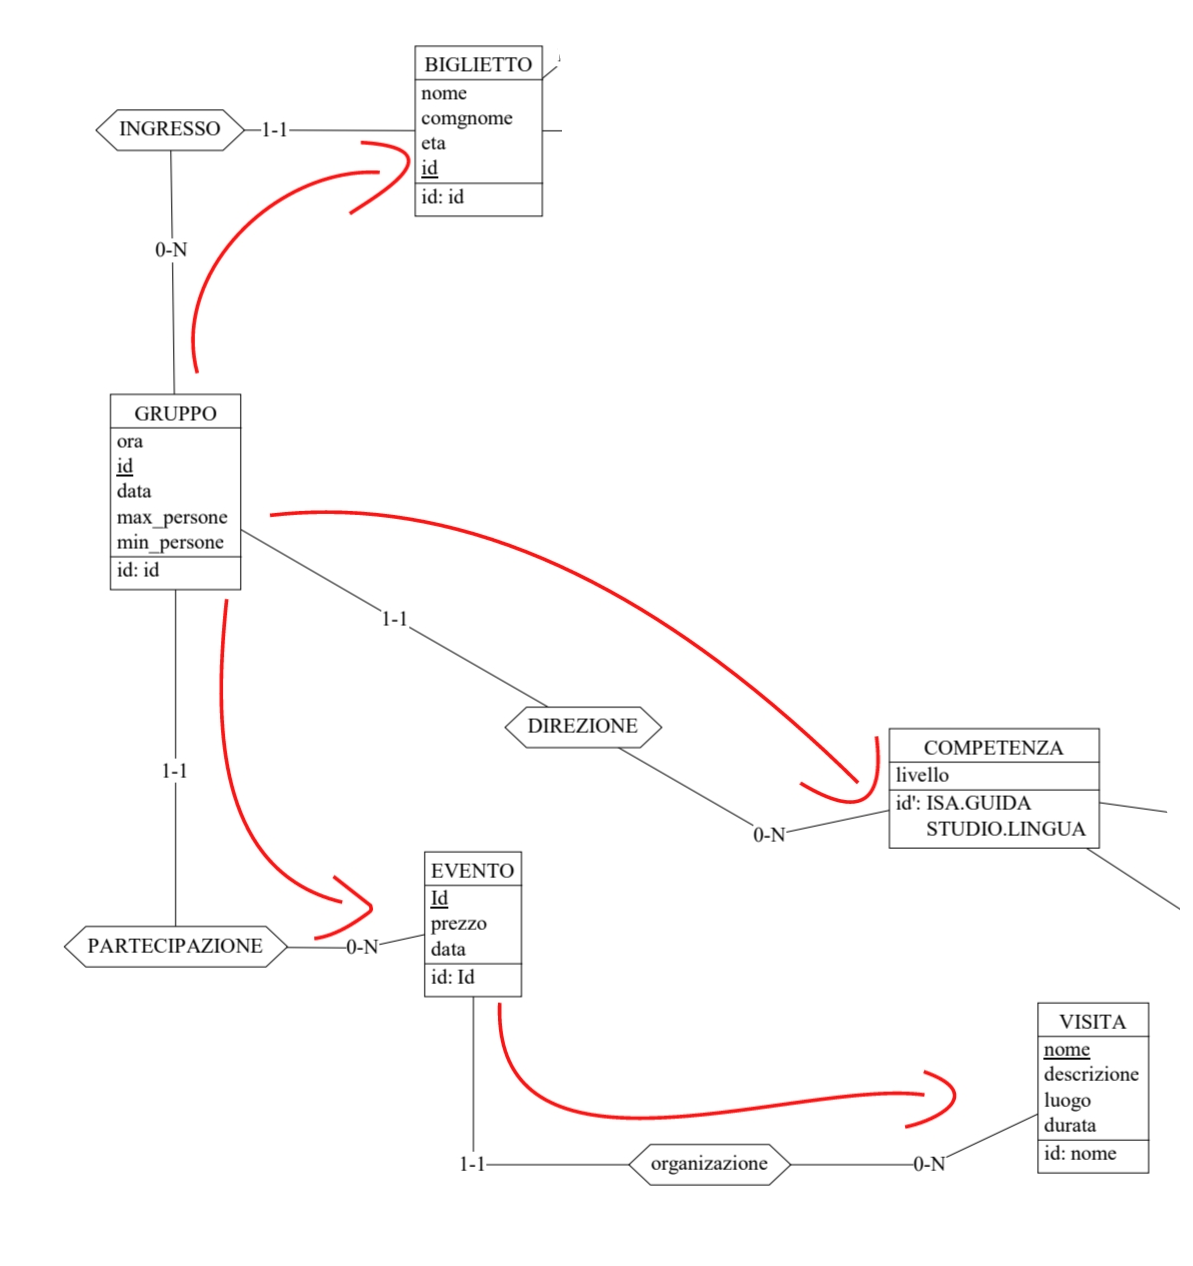
\includegraphics[width=0.9\linewidth]{schemiAccesso/inserimentoGruppo.png}
	\caption{la freccia \(EVENTO \rightarrow VISITA\) è da non considerarsi poiché evento avrà già un id di VISITA  e non sarà necessario leggerlo}
	\label{fig:aggiunta_visita}
\end{figure}
\begin{table}[H]
	\begin{tabularx}{\textwidth}{|C|C|C|C|}
		\tableheader
		\hline
		EVENTO                 & \uppercase{e}                         & \(1\) & \uppercase{l} \\
		\hline
		COMPETENZA             & \uppercase{e}                         & \(1\) & \uppercase{l} \\
		\hline
		BIGLIETTO              & \uppercase{e}                         & \(5\) & \uppercase{s} \\
		\hline
		\multicolumn{2}{|c|}{} & \multicolumn{2}{|l|}{\(TOT = 5S+2L\)}                         \\
		\hline
	\end{tabularx}
\end{table}
\subsection{Inserimento delle competenze di una guida \label{op:competenze}}
Per questa operazione bisogna ricordarsi che l'entità COMPETENZE è di tipo
debole e quindi oltre a fare una scrittura di un nuovo record bisogna anche fare
una lettura per controllare le chiavi delle entità di riferimento.
\begin{figure}
	\centering
	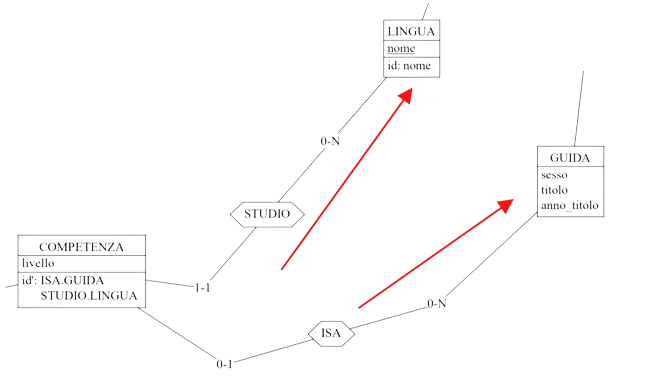
\includegraphics[width=0.9\linewidth]{schemiAccesso/COMPETENZE.png}
	\caption{Schema di navigazione per la lettura dati chiave competenza}
	\label{fig:aggiunta_competenza}
\end{figure}
\begin{table}[H]
	\begin{tabularx}{\textwidth}{|C|C|C|C|}
		\tableheader
		\hline
		COMPETENZE             & \uppercase{e}                         & \(1\) & \uppercase{s} \\
		\hline
		GUIDA                  & \uppercase{e}                         & \(1\) & \uppercase{l} \\
		\hline
		LINGUA                 & \uppercase{e}                         & \(1\) & \uppercase{l} \\
		\hline
		\multicolumn{2}{|c|}{} & \multicolumn{2}{|l|}{\(TOT = 1S+2L\)}                         \\
		\hline
	\end{tabularx}
\end{table}
\subsection{Acquisto biglietto per un determinato evento e valutazione sconto \label{op:acquisto_biglietto}}
Per l'acquisto di un biglietto bisogna controllare il gruppo a cuoi permette di
accedere e visionare l'evento di riferimento, da li è possibile risalire al
prezzo del biglietto. dopo di chè sarà possibile eventualmente valutare lo
sconto in base a all'età dell'intestatario del biglietto

\begin{figure}[H]
	\centering
	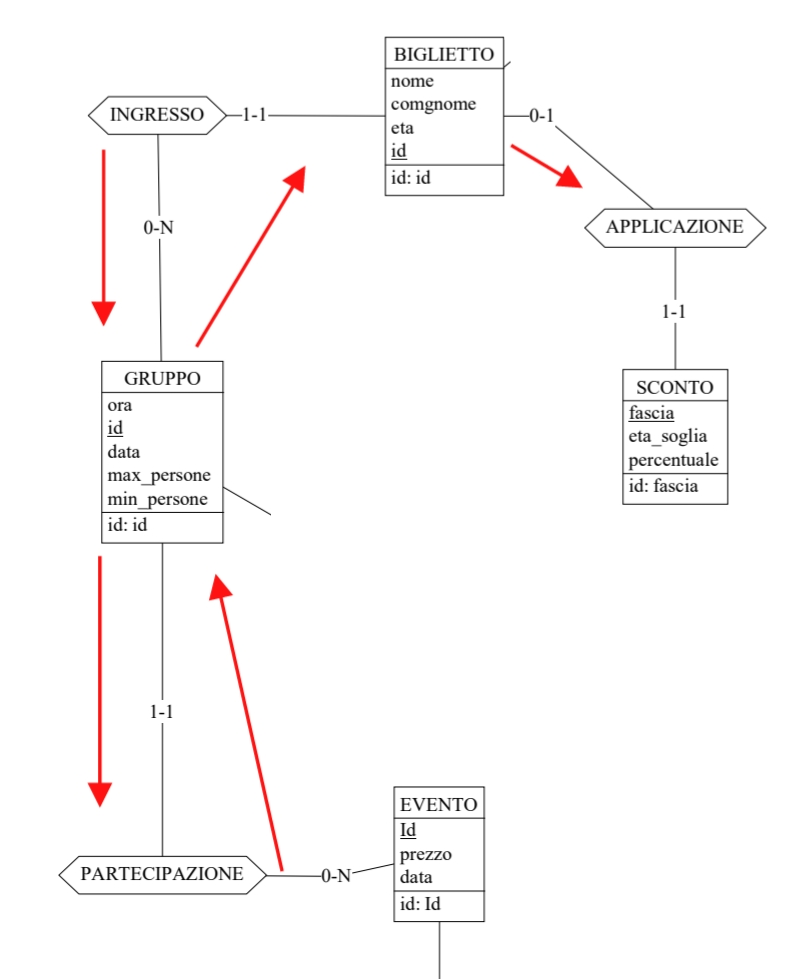
\includegraphics[width=0.9\linewidth]{schemiAccesso/ACQUISTO_BIGLIETTO.png}
	\caption{Schema di navigazione per l'acquisto di un biglietto}
	\label{fig:acquisto_biglietto}
\end{figure}

\begin{table}[H]
	\begin{tabularx}{\textwidth}{|C|C|C|C|}
		\tableheader
		\hline
		BIGLIETTO              & \uppercase{e}                         & \(1\) & \uppercase{s} \\
		\hline
		GRUPPO                 & \uppercase{e}                         & \(1\) & \uppercase{l} \\
		\hline
		EVENTO                 & \uppercase{e}                         & \(1\) & \uppercase{l} \\
		\hline
		SCONTO                 & \uppercase{e}                         & \(1\) & \uppercase{l} \\
		\hline
		\multicolumn{2}{|c|}{} & \multicolumn{2}{|l|}{\(TOT = 1S+3L\)}                         \\
		\hline
	\end{tabularx}
\end{table}
potrebbe sembrare molto macchinoso visto il volume dei dati espresso in
precedenza navigare lo schema fino ad evento per definire il prezzo del
biglietto, per tanto più avanti verrà indicato l'attributo prezzo in biglietto.
\subsection{Visualizzazione dei biglietti invenduti per un determinato evento \label{op:biglietti_invenduti}}
Per la visualizzazione dei biglietti invenduti bisogna prima controllare tutti i
biglietti associati ai gruppi dell'evento citato, dopo di che bisogna
controllare tutti i biglietti che non sono associati ad un ordine compiuto.

\begin{figure}[H]
	\centering
	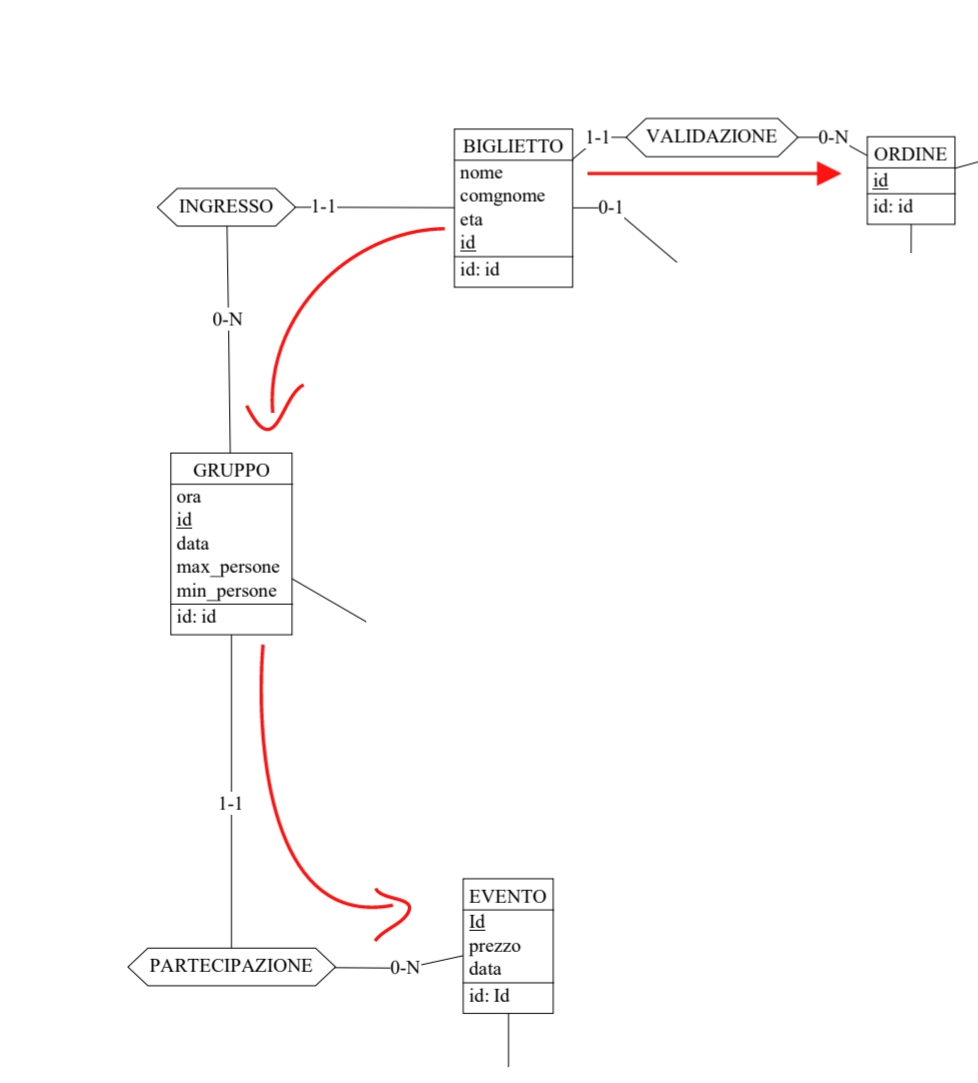
\includegraphics[width=0.9\linewidth]{schemiAccesso/BIGLIETTI_INVENDUTI.png}
\end{figure}
\begin{table}[H]
	\begin{tabularx}{\textwidth}{|C|C|C|C|}
		\tableheader
		\hline
		BIGLIETTO              & \uppercase{e}                      & \(1\) & \uppercase{l} \\
		\hline
		GRUPPO                 & \uppercase{e}                      & \(1\) & \uppercase{l} \\
		\hline
		EVENTO                 & \uppercase{e}                      & \(1\) & \uppercase{l} \\
		\hline
		ORDINE                 & \uppercase{e}                      & \(1\) & \uppercase{l} \\
		\hline
		\multicolumn{2}{|c|}{} & \multicolumn{2}{|l|}{\(TOT = 4L\)}                         \\
		\hline
	\end{tabularx}
\end{table}

\subsection{Evento che ha venduto di più a fine anno commerciale \label{op:Vendite_annuali}}
Per questa valutazione sarà necessario controllare tutti gli eventi annuali e
valutare quanti biglietti sono stati venduti per ogni gruppo e il loro prezzo.
Considerando che gli eventi hanno una frequenza di 5/mese in un anno ci sono 60
eventi, quindi per ogni evento bisogna controllare tutti i gruppi associati e
controllare quanti biglietti sono stati venduti per i relativi gruppi,
considerando quanto riferito nella tabella dei volumi in cui ad ogni evento
considero 5 gruppi quindi i gruppi annui saranno 60*5=300 a questi aggiungo un
delta maggiorativo che renda sproporzionato il conteggio in modo da avere
eventi che hanno ospitato più gruppi quindi 300+40 = 340 che sono i gruppi
annui. Faccio lo stesso ragionamento per i biglietti. E 300*5= 1500  sarebbe la
media dei biglietti annui per ogni gruppo ma devo crearli non proporzionali
quindi aggiungo di 200 biglietti in modo da avere un totale di 1700 biglietti
annui.

\begin{figure}[H]
	\centering
	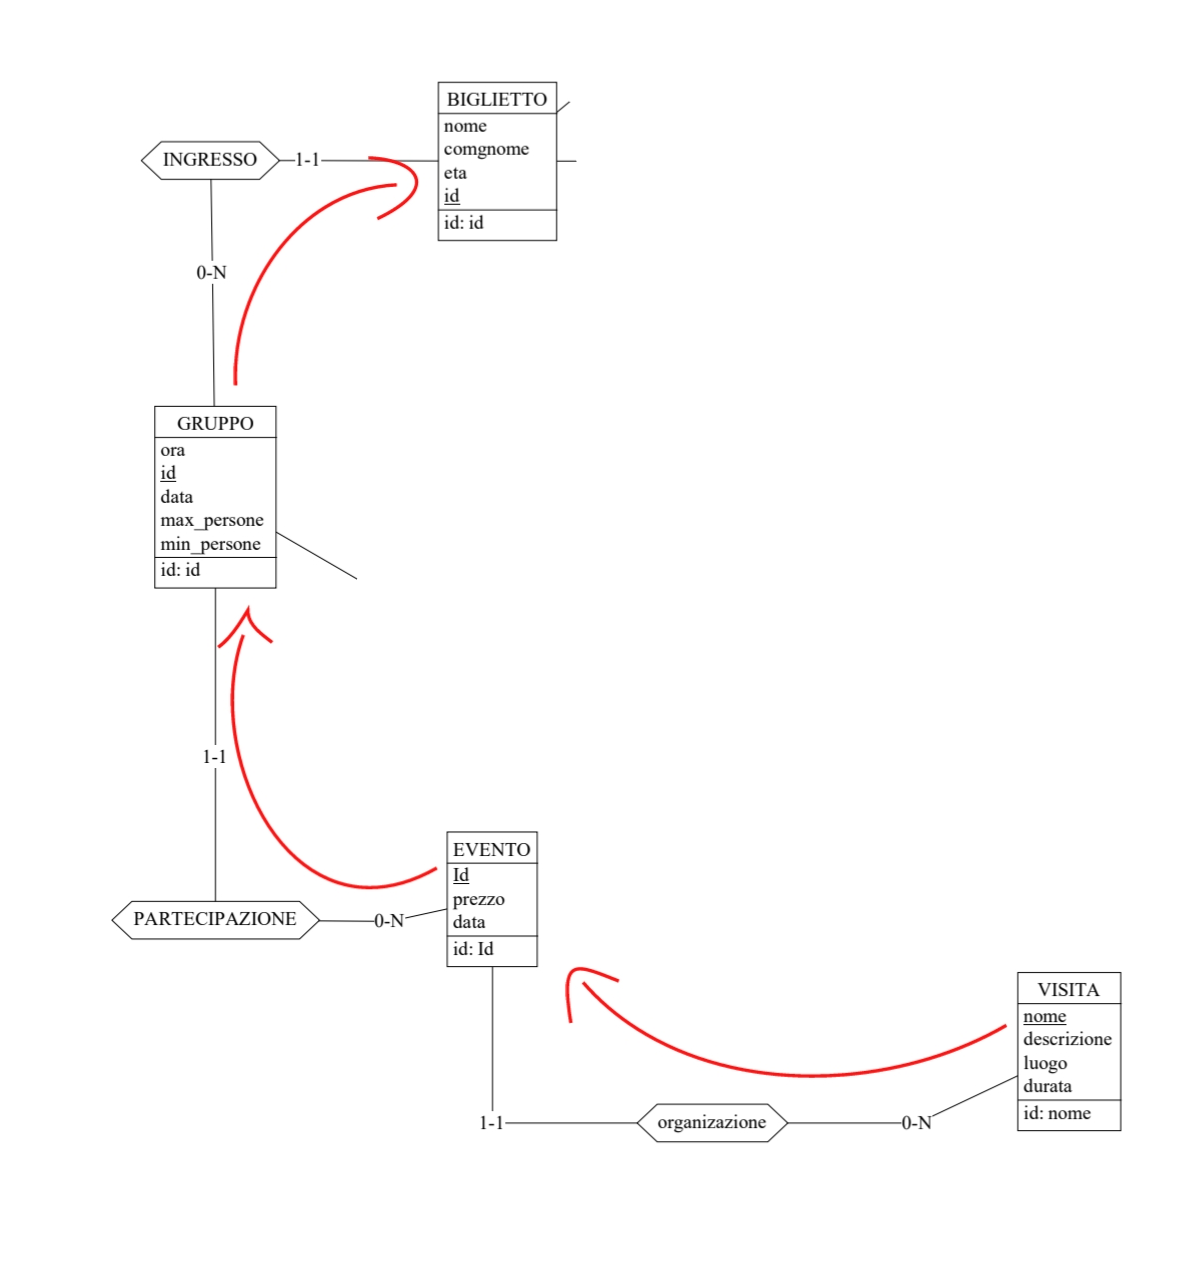
\includegraphics[width=0.9\linewidth]{schemiAccesso/venditaAnnuale.png}
\end{figure}

\begin{table}[H]
	\begin{tabularx}{\textwidth}{|C|C|C|C|}
		\tableheader
		\hline
		BIGLIETTO                         & \uppercase{e}                                   & \(1700\) & \uppercase{l} \\
		\hline
		GRUPPO                            & \uppercase{e}                                   & \(340\)  & \uppercase{l} \\
		\hline
		EVENTO                            & \uppercase{e}                                   & \(60\)   & \uppercase{l} \\
		\hline
		\multicolumn{2}{|r|}{\emph{TOT=}} & \multicolumn{2}{|l|}{\(1700L+340L+60L= 2100 \)}                            \\
		\hline
	\end{tabularx}
	\caption{Volumi per la valutazione dell'evento che ha venduto di più a fine anno commerciale}
\end{table}

alla luce delle operazioni raccolte posso aggiornare le frequenze in base alle
operazioni individuate
\begin{table}[H]
	\centering
	\begin{tabularx}{\textwidth}{|C|C|C|C|}
		\hline
		\rowcolor{red} \textcolor{white}{OPERAZIONE} & \textcolor{white}{ACCESSI}   & \textcolor{white}{FREQUENZA}                      & \textcolor{white}{ TOTALE}                         \\
		\hline
		\ref{op:Aggiunta_semplice}                   & \(1S = 2\)                   & identica alla frequenza indicata per l'operazione & moltiplicare per gli accessi la frequenza indicata \\
		\hline
		\ref{op:aggiuntaGruppo}                      & \(5S+2L = 5*2+2 =12\)        & 5/giorno                                          & \(12*5 \rightarrow 60/giorno\)                     \\
		\hline
		\ref{op:competenze}                          & \(1s+2S = 4\)                & 2/mese                                            & \(4*2 \rightarrow 8/mese\)                         \\
		\hline
		\ref{op:acquisto_biglietto}                  & \(1L+3L \rightarrow 2+3= 5\) & 3/giorno                                          & \(5*3 \rightarrow 15/giorno\)                      \\
		\hline
		\ref{op:biglietti_invenduti}                 & \(4L\)                       & 4/giorno                                          & \(4*500 \rightarrow 2000/giorno\)                  \\
		\hline
		\ref{op:Vendite_annuali}                     & \(1700L+340L+60L= 2100\)     & 1/anno                                            & \(2100*1 \rightarrow 2100/anno\)                   \\
		\hline
	\end{tabularx}
\end{table}

\section{Raffinamento dello schema}
In questa sezione mi occuperò del raffinamento dello schema concettuale
in vista della realizzazione dello schema logico. In particolare, bisogner`a
concentrarsi su una serie di operazioni.
\subsection*{Modifica degli attributi multipli e composti}
Lo schema non pensata attributi multipli o composti
\subsection*{Eliminazione delle gerarchie}
Lo schema presenta come una gerarchia quella generata da PERSONA che ha come figli CLIENTE
e GUIDA. Questa gerarchia può essere eliminata, eseguendo un collasso verso il basso,
ottenendo lo schema che segue a pagina successiva.
Oltre aver risolto la gerarchia ho provveduto a eliminare il campo presente nella relazione
CREDITO inserendolo nell'entità ordine.
\subsection*{Scelta delle chiavi}
Per le entità che posseggono più di un identificatore occorre designarne uno come
chiave primaria. In particolare.

\begin{itemize}
	\item \underline{Utente} poteva essere identificato usando come varie
	      combinazioni di attributi, ad esempio (nome, cognome, data di nascita) ho preferito
	      usare ma email per poterla sfruttare sia come chiave primaria ma anche come identificativo
	      per l'accesso al sistema informativo
	\item in \underline{Guida} è stato fatto lo stesso ragionamento
\end{itemize}

\subsection*{Eliminazioni degli identificatori esterni}
Al momento della realizzazione dello schema concettuale ho deciso omettere
direttamente attributi di entità che avrebbero dovuto raccogliere informazioni
riguardanti gli identificatori esterni lasciandoli intendere attraverso le
cardinalità delle relazioni.\\

Alla pagina seguente è possibile osservare il raffinamento dello schema con le modifiche citate.
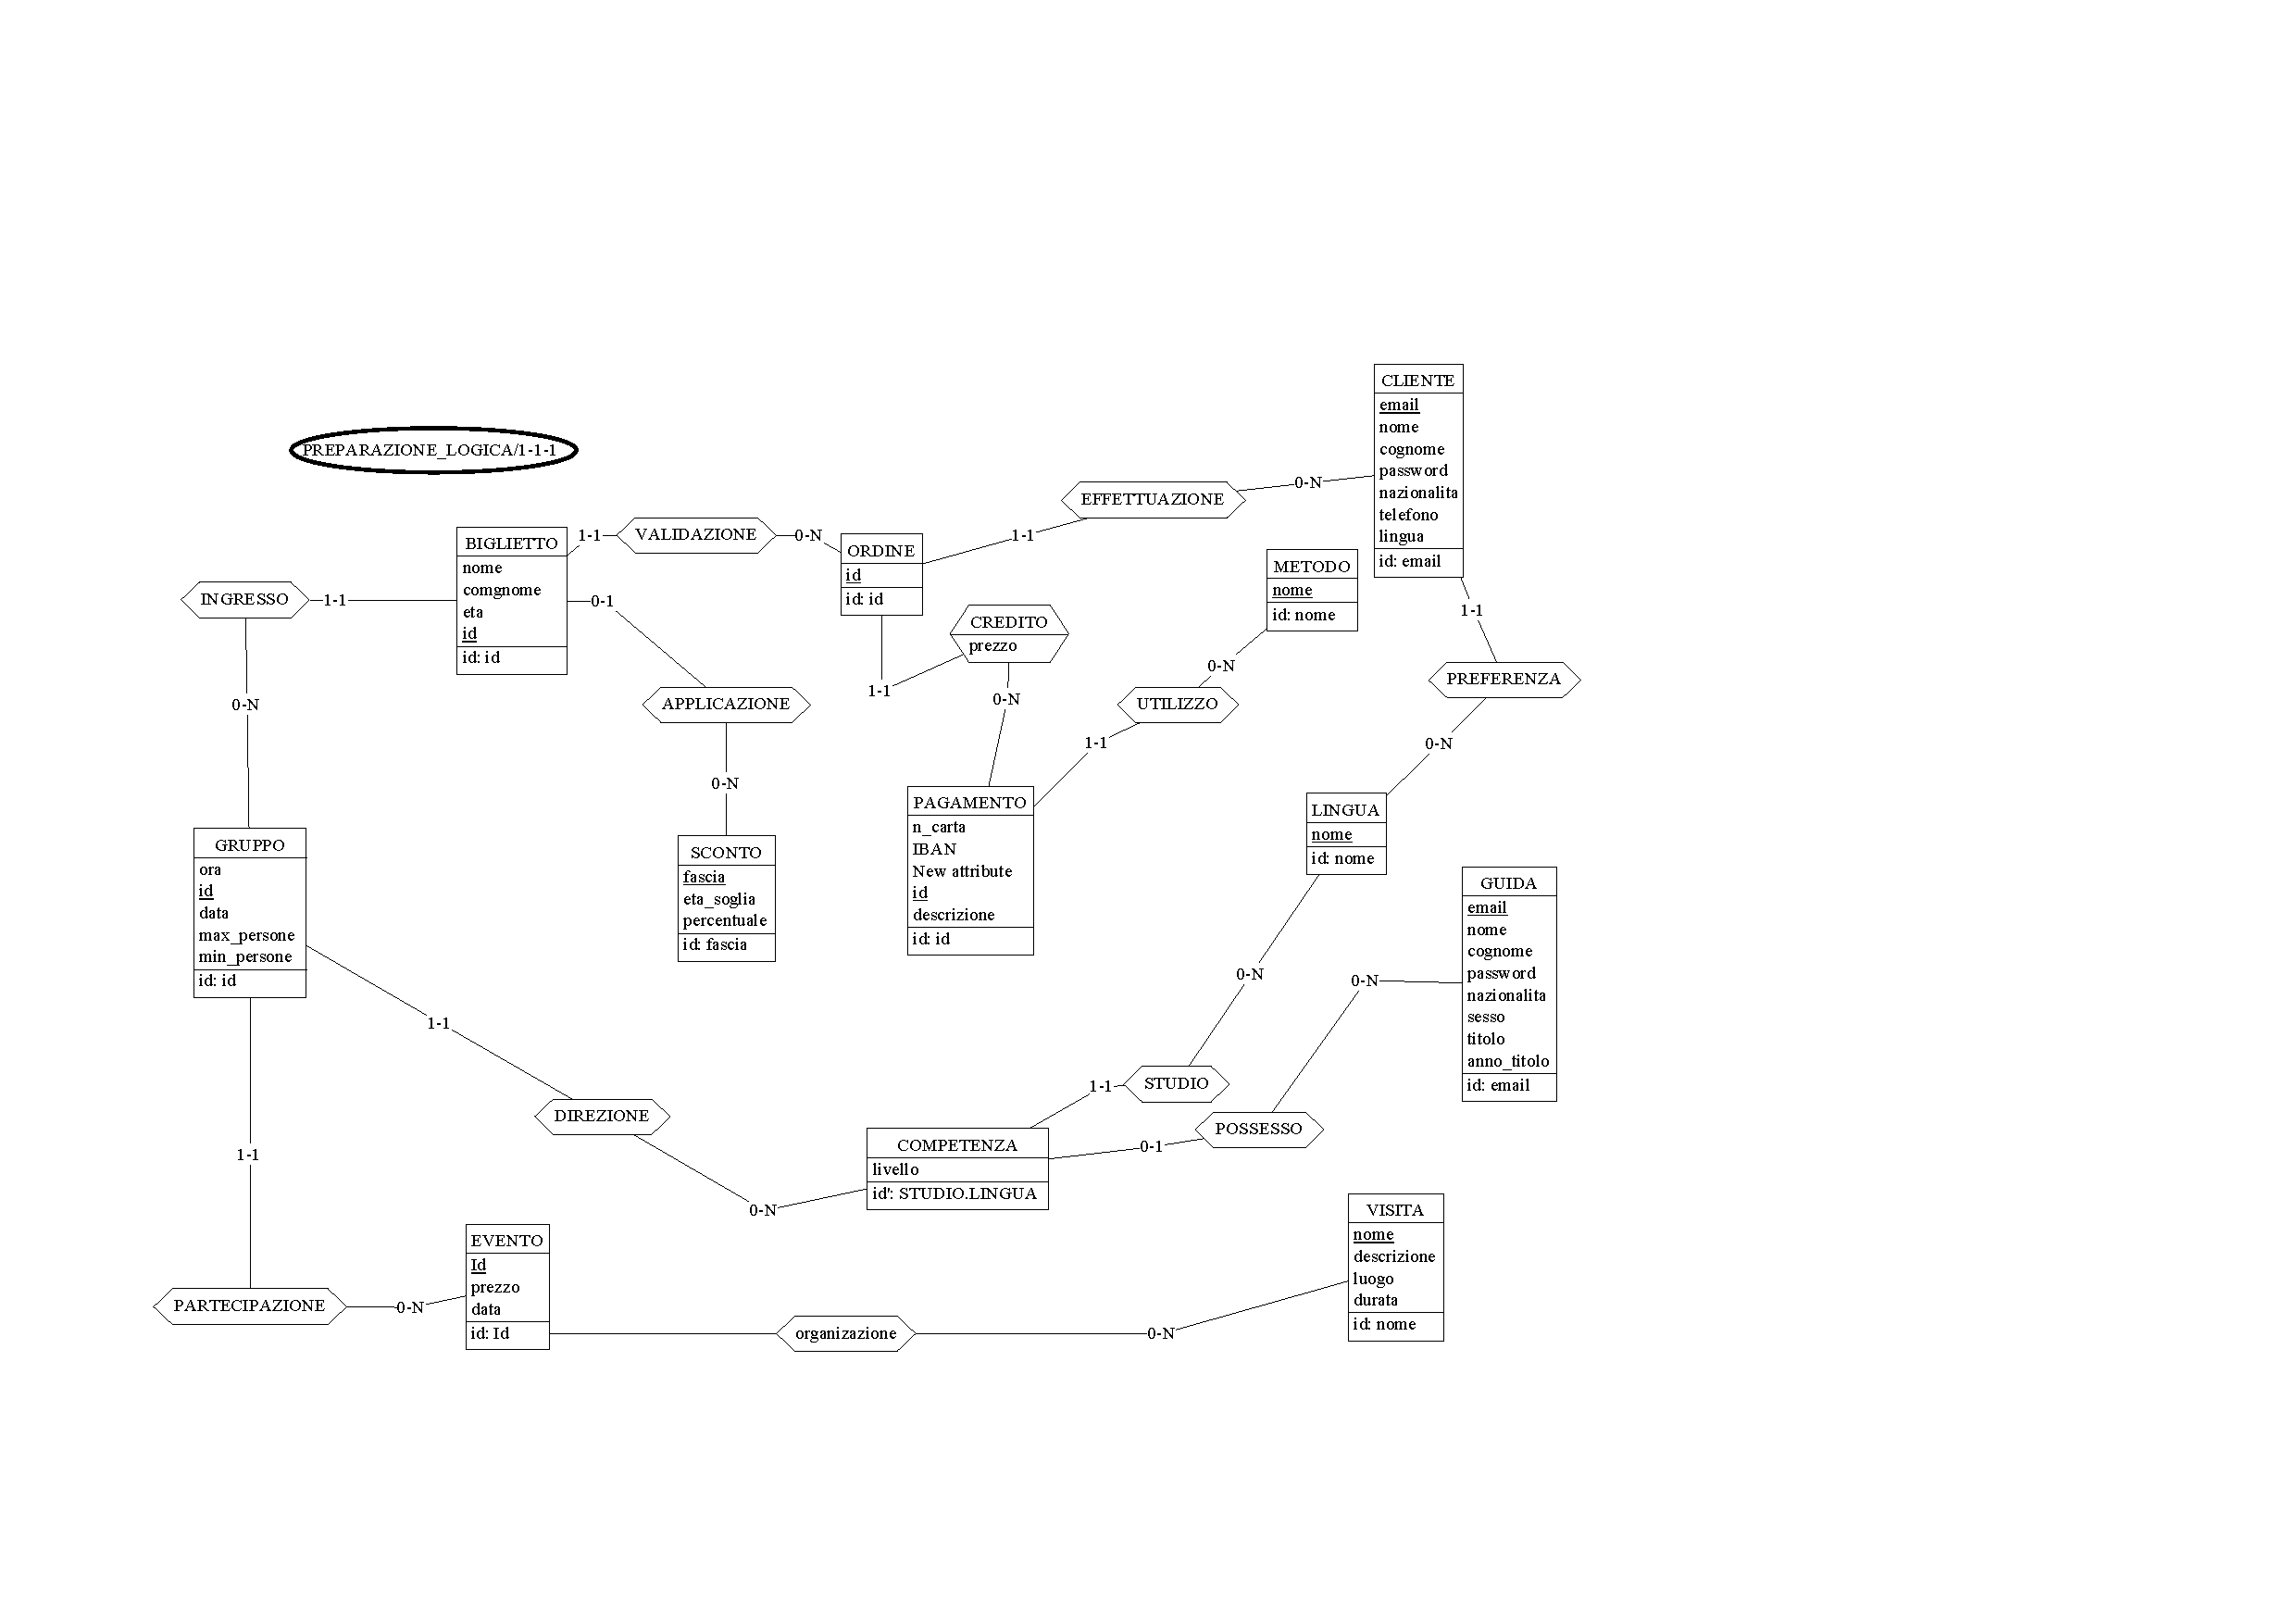
\includepdf[angle=90,pagecommand=\subsection*{Prime modifiche per lo schema logico}\thispagestyle{empty}]{../resources/pdf/Preparazione_logica.pdf}

\section{Analisi delle ridondanze}
Come già citato a momento\- della scelta dei volumi vorrei\- valutare se risulta
efficiente la presenza di ridondanze all'interno dello schema.\\ In particolare
nelle operazioni descritte risulta macchinoso dover attraversare più relazioni
per ottenere le informazioni necessarie al prezzo del biglietto per assegnare
un eventuale sconto o modificare di conseguenza l'importo totale dell'ordine.\\
Per verificarne i benefici di questa ipotesi, studiamo i casi con e senza ridondanza.

Individuo le operazioni che dipendono dalla scelta di realizzazione di tale attributo.
\begin{table}[H]
	\centering
	\begin{tabularx}{\textwidth}{|D|D|}
		\hline
		\rowcolor{red}\textcolor{white}{OPERAZIONE} & \color{white}\textcolor{white}{DESCRIZIONE}        \\
		\hline
		\ref{op:aggiuntaGruppo}                     & aggiunta di un gruppo con creazione 5 biglietti    \\
		\hline
		\ref{op:acquisto_biglietto}                 & acquisto di biglietto con valutazione dello sconto \\
		\hline
	\end{tabularx}
\end{table}
\subsection*{Valutazione operazione \ref{op:aggiuntaGruppo}}
È necessario riferirsi a quella che è la stima del volume dei dati per quanto
riguarda la frequenza di questa operazione.\\
la frequenza di questa operazione è di 60/giorno (dati presi come riferimento
alla tabella conclusiva delle frequenze)


\subsubsection*{Senza ridondanza}
i costi dell'operazione sono descritti nel paragrafo apposito
\subsubsection*{Con ridondanza}
con ridondanza bisogna notare che per scrittura di biglietto è necessario accedere al prezzo dell'evento

\begin{table}[H]
	\begin{tabularx}{\textwidth}{|C|C|C|C|}
		\tableheader
		\hline
		EVENTO                          & \uppercase{e}                                               & \(5\) & \uppercase{l} \\
		\hline
		COMPETENZA                      & \uppercase{e}                                               & \(1\) & \uppercase{l} \\
		\hline
		BIGLIETTO                       & \uppercase{e}                                               & \(5\) & \uppercase{s} \\
		\hline
		\multicolumn{2}{|c|}{}          & \multicolumn{2}{|l|}{\(TOT = 5S+6L\)}                                               \\
		\hline
		\multicolumn{2}{|c|}{ACCESSO}   & \multicolumn{2}{|l|}{\(5\times2S+6L \rightarrow 16\)}                               \\
		\hline
		\multicolumn{2}{|c|}{FREQUENZA} & \multicolumn{2}{|l|}{\(16 \times 5 \rightarrow 80/giorno\)}                         \\
		\hline
	\end{tabularx}
\end{table}

\subsection*{Valutazione operazione \ref{op:acquisto_biglietto}}
\subsubsection*{Senza ridondanza}
I costi dell'operazione sono descritti nel paragrafo apposito
\subsubsection*{Con ridondanza}

\begin{table}[H]
	\begin{tabularx}{\textwidth}{|C|C|C|C|}
		\tableheader
		\hline
		BIGLIETTO                       & \uppercase{e}                                            & \(1\) & \uppercase{s} \\
		\hline
		SCONTO                          & \uppercase{e}                                            & \(1\) & \uppercase{l} \\
		\hline
		\multicolumn{2}{|c|}{}          & \multicolumn{2}{|l|}{\(TOT = 1S+3L\)}                                            \\
		\hline
		\multicolumn{2}{|c|}{ACCESSO}   & \multicolumn{2}{|l|}{\(1\times2+3L \rightarrow 5\)}                              \\
		\hline
		\multicolumn{2}{|c|}{FREQUENZA} & \multicolumn{2}{|l|}{\(5\times3 \rightarrow 15/giorno\)}                         \\
		\hline
	\end{tabularx}
\end{table}
In ultimo, essendo SCONTO un'entità di sola lettura verrà tolta dalla relazione e sarà una entità
assestante.

\section{Traduzione di entità e associazioni in relazioni}
\subsubsection*{Legen\-da let\-tura schema logico}
\begin{itemize}
	\item I campi sottolineati rappresentano una chiava primaria \(\rightarrow\) \underline{PK}
	\item I campi con una linea tratteggiata rappresentano una chiave esterna \(\rightarrow\) \dashuline{FK}
	\item i campi che sono sia tratteggiati che sottolineati rappresentano una chiave esterna che funge da chiave primaria \(\rightarrow\) \underline{\dashuline{FK+PK}}
\end{itemize}
Dove compaiono chiavi esterne sono riportate le relazioni a cui fanno riferimento.\\\\
\fbox{
	\begin{minipage}{\textwidth}
		CLIENTE(\underline{email}, nome, cognome, password, nazionalita, telefono, \dashuline{lingua})\\
		\textit{FK: lingua REFERENCES LINGUE}
		LINGUA(\underline{nome})\\
		GUIDA(\underline{email} ,nome, cognome, password, sesso, titolo, anno\_titolo)

	\end{minipage}
}



\section{Schema relazionale finale}
\newpage
\section{Traduzione delle operazioni in query SQL}
% \begin{lstlisting}[style=codeStyle,language=SQL]
% 	CREATE TABLE `competenze` (
%   	`id_guida` int(11) NOT NULL,
%   	`lingua` varchar(15) NOT NULL,
%   	`livello` varchar(15) DEFAULT NULL
% ) ENGINE=InnoDB DEFAULT CHARSET=utf8mb4 COLLATE=utf8mb4_general_ci;
% \end{lstlisting}
\lstinputlisting[style=codeStyle, language=SQL]{../../SQL/visite_turistiche.sql}

\newpage
\chapter{Progettazione dell'applicazione}
\end{document}
